
\documentclass[10pt]{proc}
\usepackage{hyperref}
\usepackage{mathtools}
\usepackage{amsmath}
\begin{document}

\large{\textbf{SWIM through the NATs}}\\

\large{\textbf{Authors: Mattias Cederlund, Joakim af Sandeberg}}

\section{Introduction}
The project consisted of implementing, testing and evaluating a decentralized group membership service called SWIM. A skeleton codebase was given as an outline for the program. The assignment had two parts. The first was to implement SWIM as stated in the paper  and the second part was to extend it so it works in a NATed environment. 
\section{Main problems}
The application had four main problems that needed to be addressed:
\begin{itemize}
\item Pings and indirect pings.
\item Membership discovery and piggybacking.
\item Incarnation counters and alive messages.
\item Making the application support NAT.
\end{itemize}

\subsection{Pings and indirect pings}
Implementing pings and indirect pings (K-pings) was very straight forward. A ping message is sent to a random peer and a timer is started. If a pong message is returned before the timer runs out the peer is considered to be alive. Otherwise it is either considered dead (basic failure detection) or suspected after indirect pings are sent to it (as stated in the SWIM paper). 
\\[10pt]
Indirect pings are sent via the sender's other alive peers. These peers just relay the ping to the target and relays the pong back to the sender. If none of the indirect pings make it the peer is added to the suspected list, to be declared dead later on.
\subsection{Membership discovery and piggybacking}
Each node keeps a send buffer of recent newly added, suspected and dead peers. These values are coupled with a counter of how many times they have been sent. When the peer responds to a pong it takes the information from the buffer with the lowest counters and adds them to the response. If any of these values has been sent \(\lambda *log(n)\) times they are removed from the buffer. If a node receives a ping from a node not yet discovered it is added as a new alive node in the buffer.
\subsection{Incarnation counters and alive messages}
Each node has an incarnation counter. If it discovers itself in any nodes suspected list it increases its incarnation counter and sends an alive message to all alive nodes that it knows of. This hopefully purges it from the suspected lists and decreases the chance of functioning nodes being marked as dead in the system.
\subsection{Making the application support NAT}
To make the application support NATs the NAT component is extended to send heartbeats to all nodes that is considered its parents. If a parent does not respond to the heartbeat in time it is considered dead and a new parent is retrieved from the sample provided by Croupier. It then sends a message to the SWIM component, notifying it has received new parents. The SWIM component adds itself to the send buffer with its new parents and the new address for the node is propagated via the regular piggybacking in the SWIM component.
\section{Tests and evaluation}
The following chapter describes the tests and evaluation that were done. All tests were run 10 times and an average is displayed if nothing else is mentioned. Standard deviation is shown at the 95\% and 5\% interval on the bar graphs.
\subsection{Swim and scenario parameters}
Parameters for the SWIM implementation is defined as constants at the top of SwimComp. The three main parameters are:
\begin{itemize}
\item K - How many indirect pings should be sent if a direct ping fails.
\item PIGGYBACK\_MESSAGE\_SIZE - How many node changes are piggybacked in each pong message.
\item LAMBDA - How many times each node change is piggybacked. (LAMBDA * log(n))
\end{itemize}
Parameters for the test cases are found at the top of SwimMain. The parameters are:
\begin{itemize}
\item USE\_RANDOM\_SEED - If set to true a random seed will be used for the simulation, otherwise 1234 will be used.
\item SIMULATION\_LENGTH - Length of simulation in cycles (1 ping is sent per cycle)
\item NUMBER\_OF\_NODES - How many nodes should participate in the simulation.
\item BOOTSTRAP\_SIZE - How many nodes each node should be given at bootstrap. Was set to 5 in the provided code.
\item ALLOW\_NAT - If set to true some of the nodes will be behind NATs.
\item NATED\_NODE\_FRACTION - Sets the ratio of NATed nodes as 1/NATED\_NODE\_FRACTION. A value of 2 gives 50\% NATed nodes, 3 gives 33\% etc.
\item KILL\_SIZE - If simulating with failure, this is the total number of nodes which should fail during the simulation.
\item KILL\_INTERVAL - How often the nodes should fail, in cycles.
\item FAILURE\_AFTER - How long to wait before nodes begin to fail.
\end{itemize}
For each test presented below we will provide the interesting parameters used so it can be reproduced. For all tests K will be set to 4 and LAMBDA will be set to 3.
\\[10pt]
In the project there also exists other parameters, such as various timeouts, but these are never changed between the test cases and should be assumed to be the same as in the source code.
\subsection{Convergence calculation}
All nodes report their current alive, suspected and dead nodes every cycle. This data is stored and after execution the convergence is calculated. 
\\[10pt]
We calculate convergence by extracting the nodes which are common to all nodes and divide it by the total number of unique nodes that are found in all alive lists. This calculation method will give a very strict measure of the convergence, but it also opens up for some problems with misleading values. For example, if one single node in the entire system ends up with 0 nodes in its alive list, the convergence for the entire system will be calculated as 0, even though all other nodes may be 100\% converged. 
\\[10pt]
Some graphs uses median value instead of average. This is because the graphs is more representative this way. With median the graph appears to be fully converged when 50\% of the test runs have converged instead of all runs. If average was used the graph would seem to show the worst case scenario.
\subsection{Without NATed nodes}
As seen in Figure 1, the nodes converge quickly thanks to the unbounded message size. The number of nodes does not affect the result much.
\\[10pt]
Figure 2 shows the result when testing bootstrap convergence with 50 nodes and varying message size. The message size is affecting the performance a lot as the piggybacking can not be done efficiently if it is set too low. With infinite message size the nodes converge after only 11 cycles and with 6 (as used in the SWIM paper) it takes 46 cycles.
\begin{figure}[h!]
\centering
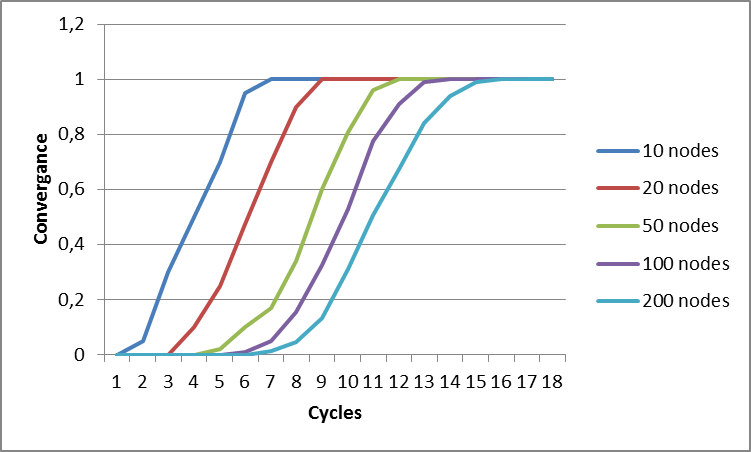
\includegraphics[width=0.5\textwidth]{Fig1.png}
\caption{\label{fig.1}Bootstrap convergence. Message size unbounded, bootstrap size 2. The lines show median value.}
\end{figure}
\begin{figure}[h!]
\centering
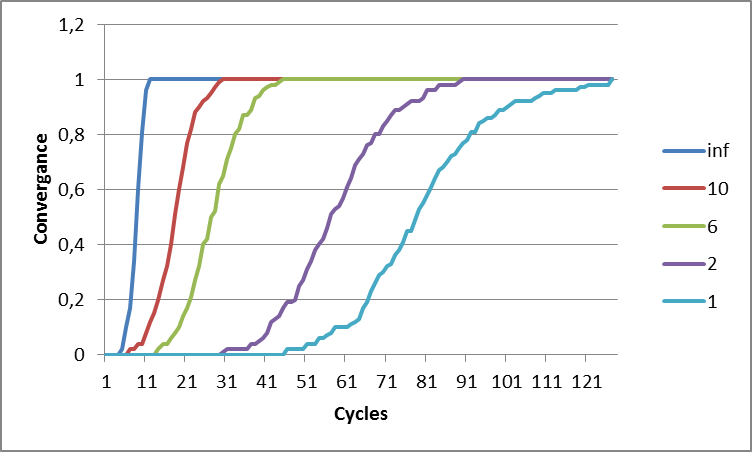
\includegraphics[width=0.5\textwidth]{Fig2.png}
\caption{\label{fig.2}Bootstrap convergence. 50 nodes, bootstrap size 2. The lines show median value.}
\end{figure}
\begin{figure}[h!]
\centering
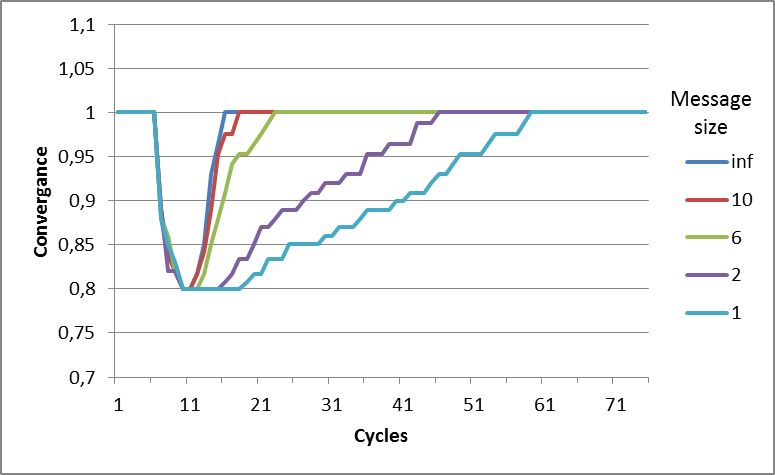
\includegraphics[width=0.5\textwidth]{Fig3.png}
\caption{\label{fig.3}Convergence after catastrophic failure (20\% of nodes fail). 50 nodes. The lines show median value.}
\end{figure}
\begin{figure}[h!]
\centering
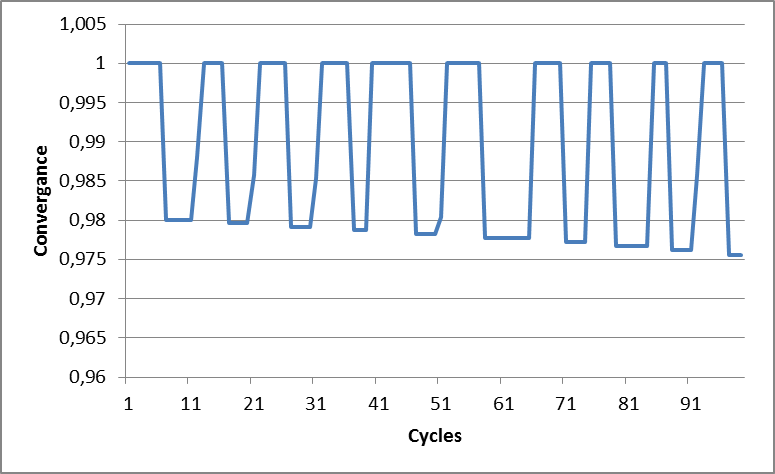
\includegraphics[width=0.5\textwidth]{Fig4.png}
\caption{\label{fig.4}Convergence during churn. One node deaths every 10 cycles. 50 nodes.}
\end{figure}
\\[10pt]
In Figure 3 we tested how SWIM reacts to catastrophic failure. 20\% of the nodes fail at the same time and the graph is showing how the nodes converges afterwards. With the current settings, it takes the nodes 6 cycles to mark a node as dead. In the graph the nodes die at cycle 0 and detection begins at cycle 6. The performance is yet again affected a lot by the message size, where infinite message size gives almost instantaneous recovery and for a message size of 6 it takes 25 cycles to recover.
\\[10pt]
In Figure 4 we present how the system behaves during churn of 1 node death every 10 cycles. This was only tested with unbounded message size, as the node changes would not fill the send buffer anyway, unless using unrealistically small message sizes. The system is fully recovered  4-6 cycles after the failure was detected.
\\[10pt]
Tests were also performed with link deaths. With 50 nodes we killed 100 random links and the convergence of the system was not affected at all. The system thus handles link deaths with good results, thanks to the indirect pings. With a K value high enough (tested with 4) the risk of selecting only nodes with disconnected links is low. The graph of this execution was omitted from the report.
\subsection{With NATed nodes}
The exact same tests we performed without NATed nodes were also executed with NATed nodes enabled. For all tests 50\% of the nodes were behind NATs.
\\[10pt]
\begin{figure}[h!]
\centering
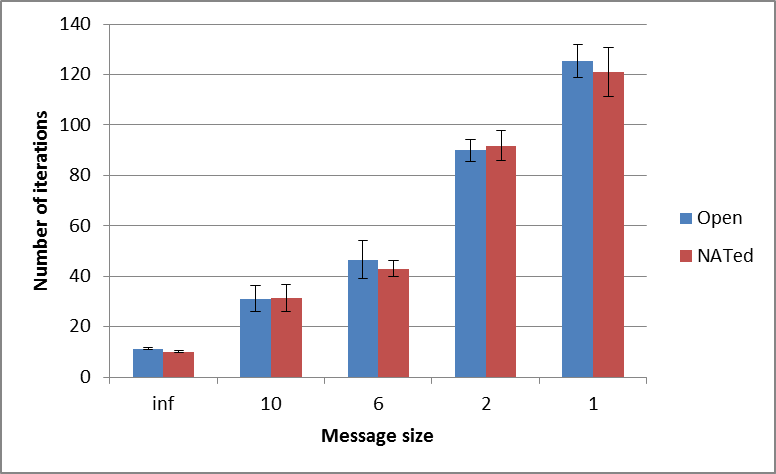
\includegraphics[width=0.5\textwidth]{Fig5.png}
\caption{\label{fig.5}Bootstrap convergence. 50 nodes. Bootstrap size 2. Comparison between 100\% open and 50\% NATed nodes. Bars show a 95\% standard deviation.}
\end{figure}
\begin{figure}[h!]
\centering
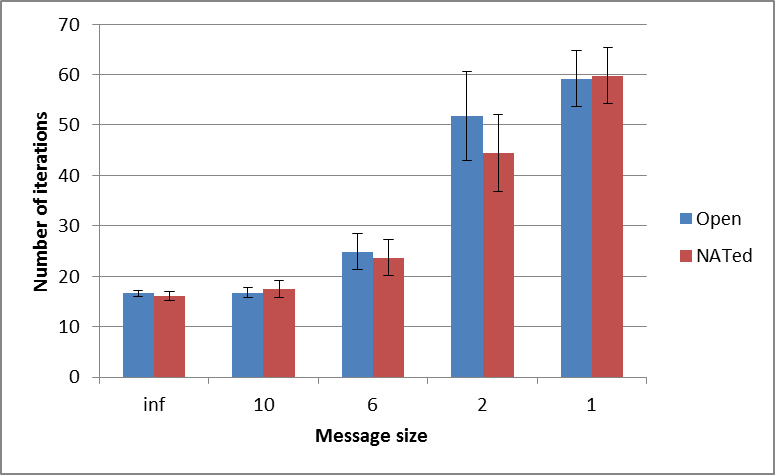
\includegraphics[width=0.5\textwidth]{Fig6.png}
\caption{\label{fig.6} Convergence after catastrophic failure (20\% of nodes fail). 50 nodes. Comparision between 100\% open and 50\% NATed nodes. Bars show a 95\% standard deviation.}
\end{figure}
\\[10pt]
When we tested the bootstrap convergence with 50\% NATed nodes we got similar results as for 100\% open nodes. The comparison can be seen in Figure 5. 
\\[10pt]
Figure 6 is showing the comparison when testing catastrophic node deaths (20\% of nodes fail). These results were also very similar to the 100\% open case. When we increased the failure rate to 40\% we sometimes had good results where the system managed to recover fully, but every now and then it did not. We located the cause of the problem to the Croupier samples. Sometimes Croupier returned empty samples, so when the parents of a NATed node died it would not get any new parents. This caused all pongs to the node to fail and thus the node would mark all other nodes as dead. With our strict convergence calculation this resulted in 0 in convergence rate.
\\[10pt]
\begin{figure}[h!]
\centering
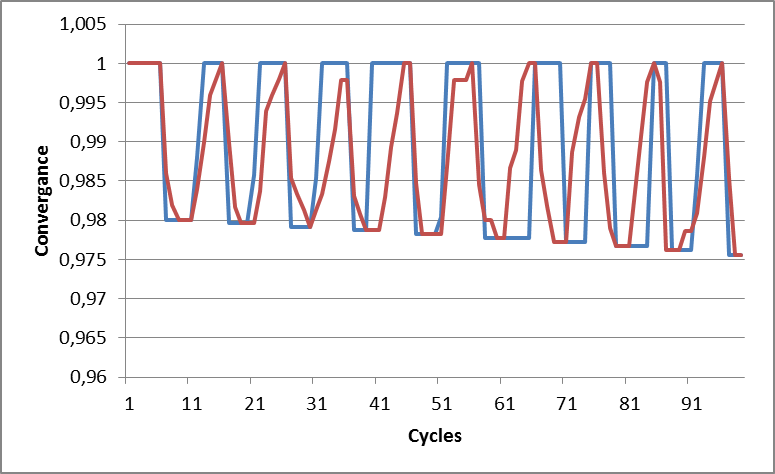
\includegraphics[width=0.5\textwidth]{Fig7.png}
\caption{\label{fig.7}Convergence during churn. One node dies every 10 cycles. 50 nodes. Comparison between 100\% open and 50\% NATed nodes.}
\end{figure}
\\[10pt]
Also the churn test had similar results. The main difference, although hard to visualize, was that the time to converge varied more making the NATed system less predictable. It also averaged at a slightly lower convergence rate, as seen in Figure 7.
\subsection{Test on network delay}
Some tests were run with network delay and the system should be able to handle network delay up to 1/4th of the timeout of the pings. This is because the pings could need up to 4 hops (node to parent, parent to child, child to parent, parent to node) between sending a ping and receiving a pong. 
\\[10pt]
The delay was most important to have right in the NatTraversalComp since the heartbeat ping does not have any suspicion mechanism and would report deaths more frequently. 
\\[10pt]
When the tests were executed with network delay Croupier started providing empty samples so NATed nodes were not always able to receive new parents. This meant that some NATed nodes were declared dead even though they had not crashed.
\subsection{Test of different lambdas}
We did tests with lambda values of 4, 3, 2 and 1, with bootstrap size 2, infinite message size and 50 nodes in the system. The start up time for lambda at 4 and 3 were as good as identical as both took an average of 13,4 cycles to converge. A lambda of 2 performed slightly worse than 4 and 3 but still rather close with 14,9 cycles instead. With lambda set to 1 the time to converge was 10 times as long with an average of 146,5 iterations and the standard deviation was 50 times higher showing a great spread in convergence time. This means that lambda\(>\)1 should be used since the performance suffers greatly at lambda = 1.
\subsection{Discussion of the tests}
The tests presented were done without any network delay. This means that the results are more uniform and better than those of a real world system. 
\\[10pt]
The tests were all done with either a bootstrap size of 2 (startup tests and churn) or 4 (failure tests). How the system performs for other bootstrap sizes were not evaluated.
\\[10pt]
The tests on NATed nodes were all done with 50\% NATed node. This was what we felt as an upper bound for amount of NATed nodes (especially for the failure tests if open nodes crash as often as NATed) and results with a lower ratio should perform in between the results of the NATed tests and the open tests.
\section{Conclusion}
This report has summarized the implementation and evaluation of SWIM, where we enabled support for NAT traversal. We have through the evaluation showed that the system converges quite quickly and is also performs well when failures are present in the system.
\subsection{Thoughts on the assignment}
The assignment served as a good example on how to implement a decentralized group membership and fitted nicely into the course. It also showed the importance of taking NAT into account when constructing a distributed system. It was hard to fit all possible tests into the report since so many different configurations could be made, thus this report only covers the most important and most basic tests.
\clearpage
\appendix
\section{Source code}
The source code is available on GitHub: \url{https://github.com/jotunacorn/id2210-vt15}
\\[10pt]
Instructions on how to run the tests are provided in a README file.
\section {Data from the tests}
Data from the tests are available as Excel format. (.xlsx) here:
\url{https://www.dropbox.com/s/j4jhmkupfzxc02k/Bif%20sample%20size.xlsx?dl=0}
\begin{figure}[h!]
\centering
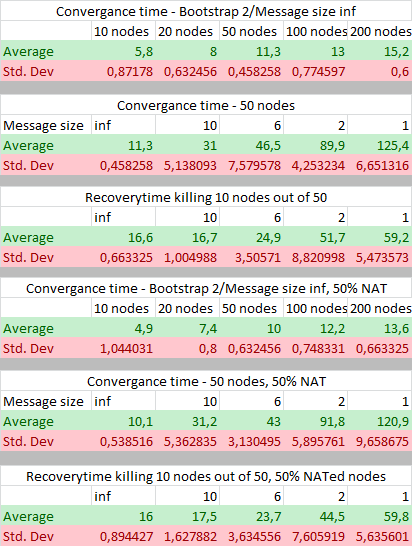
\includegraphics[width=0.6\textwidth]{tests.png}
\caption{\label{fig.8}A sample of results from the Excel file.}
\end{figure}
\end{document}
